% ======================================================================
\section{Visión general}
El presente documento constituye el modelo de comportamiento del sistema.

Partiendo de los casos de usos se presentan los diagramas de secuencias que modelan 
los eventos que el sistema puede recibir del usuario y los valores de retorno
que produce como consecuencia de estos.  Esta sección considera tanto al sistema intérprete
como el cliente.

A partir de los diagramas de secuencia del sistema se obtienen las operaciones 
que este presenta. Luego se describen los contratos de cada una de las operaciones.  
% ======================================================================
\section{Diagramas de secuencia del sistema}
\subsection{Intérprete}
\subsubsection{Interpretar entrada estándar}
\begin{center}
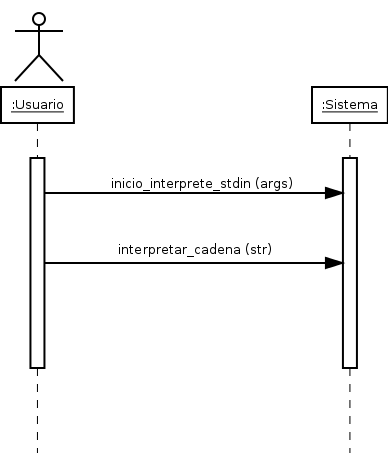
\includegraphics[scale=0.4]{interpretar_stdin.png} \\
\end{center}

\subsubsection{Interpretar línea}
\begin{center}
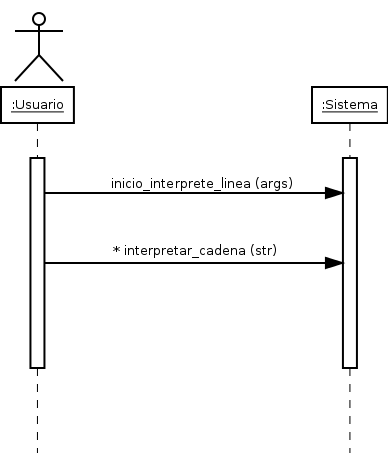
\includegraphics[scale=0.4]{interpretar_line.png} \\
\end{center}

\subsubsection{Interpretar fichero}
\begin{center}
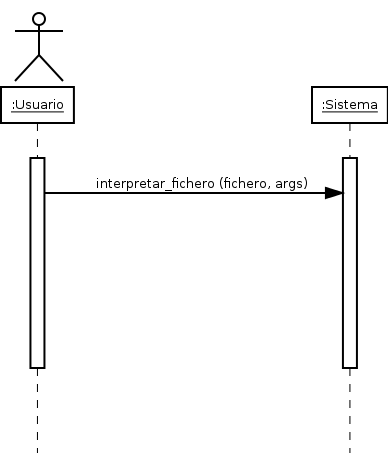
\includegraphics[scale=0.4]{interpretar_file.png} \\
\end{center}

\subsubsection{Ver ayuda}
\begin{center}
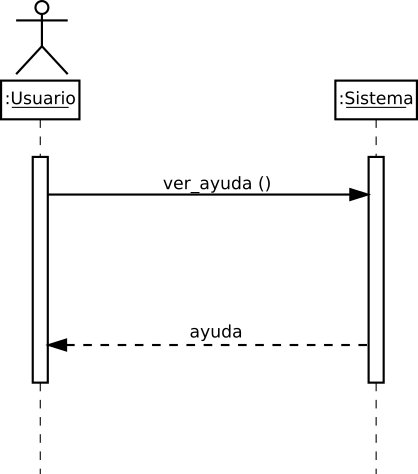
\includegraphics[scale=0.4]{ver_ayuda.png} \\
\end{center}

\subsubsection{Cargar extensión}
\begin{center}
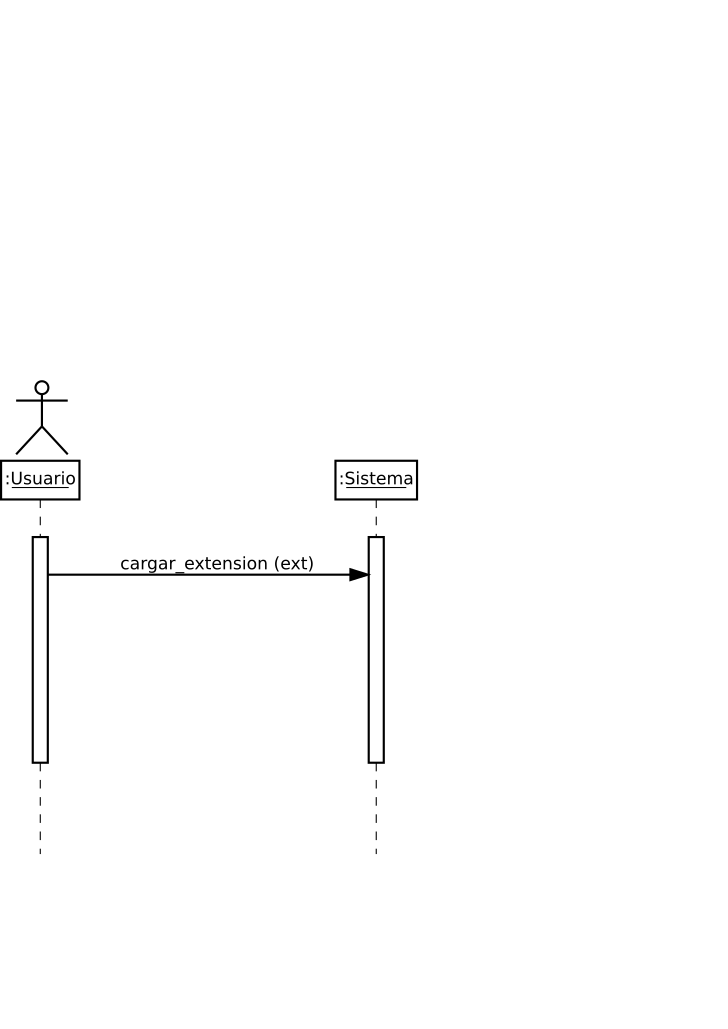
\includegraphics[scale=0.4]{cagar_extension.png} \\
\end{center}

\subsubsection{Listar extensiones}
\begin{center}
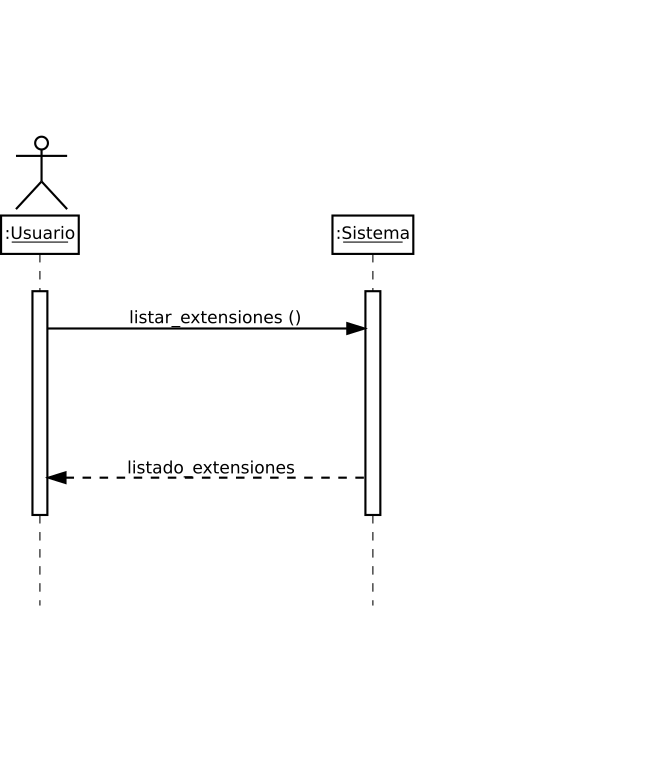
\includegraphics[scale=0.4]{listar_extensiones.png} \\
\end{center}

\subsubsection{Iniciar interpretación red}
\begin{center}
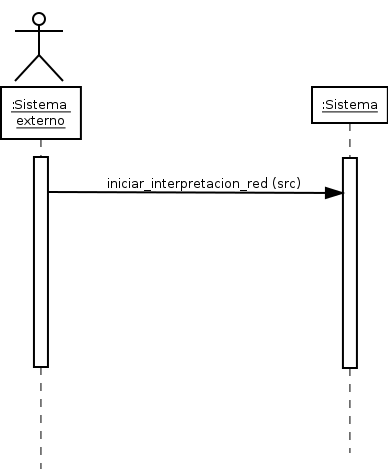
\includegraphics[scale=0.4]{iniciar_interpretacion_red.png} \\
\end{center}

\subsubsection{Obtener pasos interpretación red}
\begin{center}
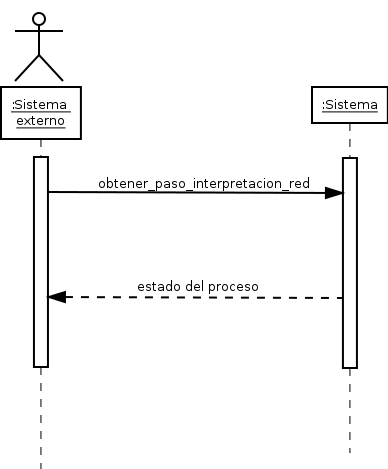
\includegraphics[scale=0.4]{obtener_paso_interpretacion_red.png} \\
\end{center}


\subsection{runTree}
\subsubsection{Enviar código fuente}
\begin{center}
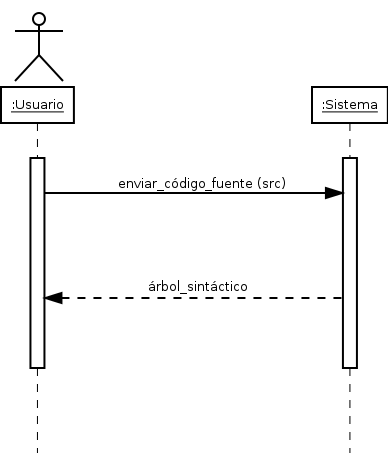
\includegraphics[scale=0.4]{enviar_codigo_fuente.png} \\
\end{center}
\subsubsection{Siguiente paso}
\begin{center}
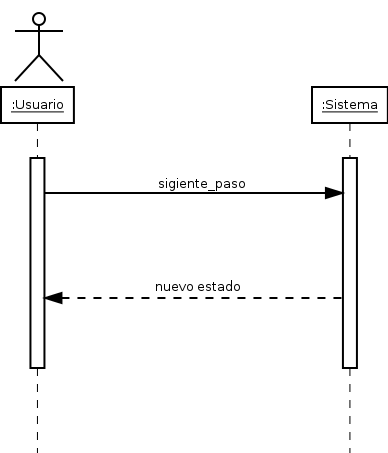
\includegraphics[scale=0.4]{siguiente_paso.png} \\
\end{center}
\subsubsection{Siguiente sentencia}
\begin{center}
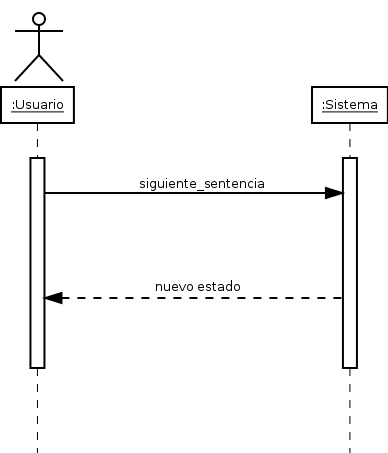
\includegraphics[scale=0.4]{siguiente_sentencia.png} \\
\end{center}
\subsubsection{Activar ejecución automática}
\begin{center}
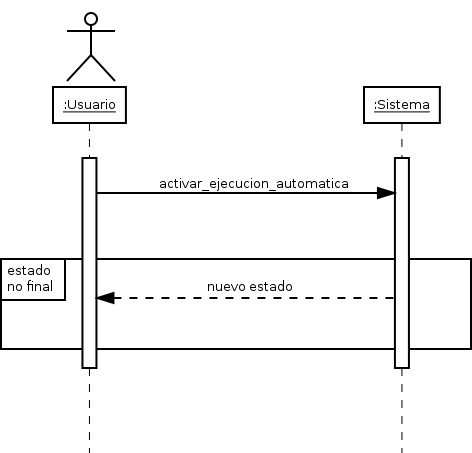
\includegraphics[scale=0.4]{activar_ejecucion_automatica.png} \\
\end{center}
\subsubsection{Desctivar ejecución automática}
\begin{center}
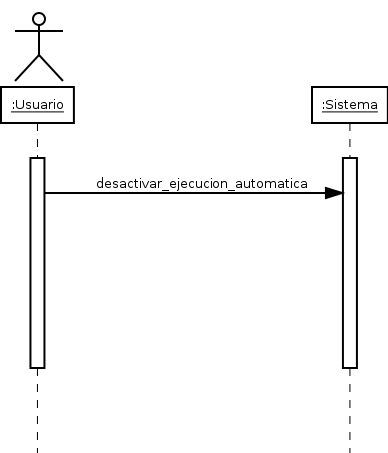
\includegraphics[scale=0.4]{desactivar_ejecucion_automatica.png} \\
\end{center}
\subsubsection{Limpiar salida}
\begin{center}
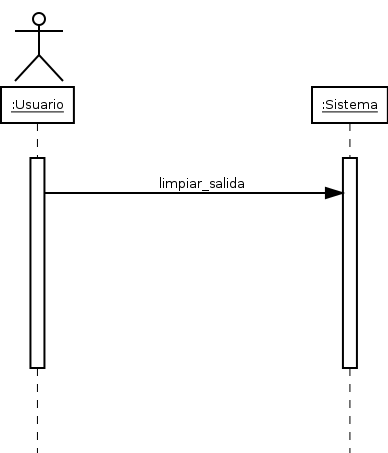
\includegraphics[scale=0.4]{limpiar_salida.png} \\
\end{center}
\subsubsection{Ver infomación de nodo}
\begin{center}
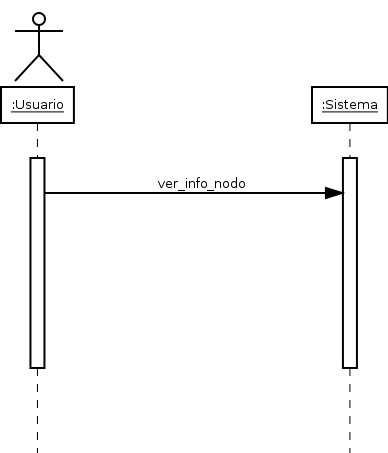
\includegraphics[scale=0.4]{ver_info_nodo.png} \\
\end{center}
\subsubsection{Ver contenido tabla de símbolo}
\begin{center}
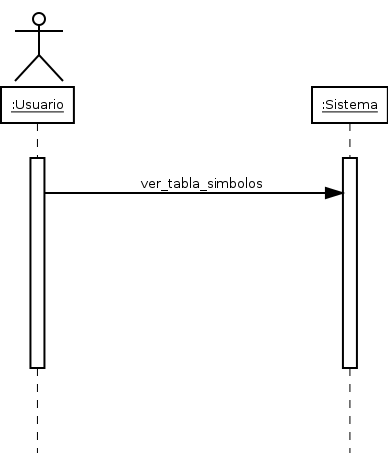
\includegraphics[scale=0.4]{ver_tabla_simbolos.png} \\
\end{center}
\subsubsection{Guardar código fuente}
\begin{center}
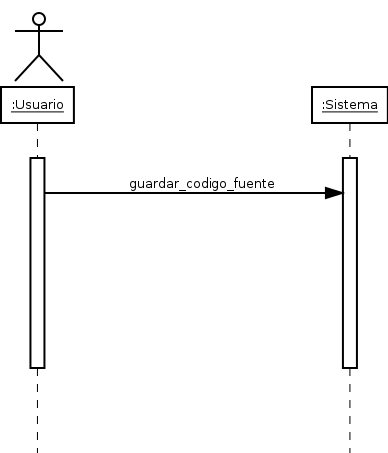
\includegraphics[scale=0.4]{guardar_codigo_fuente.png} \\
\end{center}
\subsubsection{Abrir código fuente}
\begin{center}
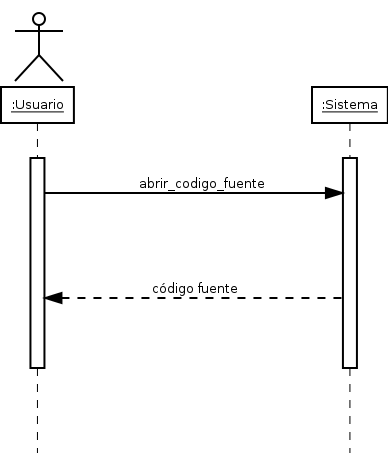
\includegraphics[scale=0.4]{abrir_codigo_fuente.png} \\
\end{center}

\section{Contratos de operaciones del sistema}
En esta sección se listan las operaciones del sistema y se detallan los contratos de aquellas
que implican un cambio en la estructura de datos interna del programa. 

\subsection{Intérprete}
\begin{center}
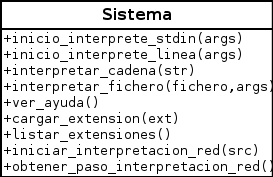
\includegraphics[scale=0.7]{operaciones_sistema.png} \\
\end{center}
\subsubsection{Operación inicio\_interprete\_stdin}

	\begin{description}
		\item [Nombre:] inicio\_interprete\_stdin(args)
		\item [Responsabilidades:] Iniciar la interpretación de la entrada estándar.
		\item [Referencias Cruzadas: ] Caso de Uso: Interpretar entrada estándar
      \item [Precondiciones:] No tiene.
      \item [Postcondiciones:] \hfill
      \begin {itemize}
         \item Se creó una instancia ``i'' de ``interpreter'' (creación de objeto).
         \item Se inicializaron los atributos de ``i''.
         \item Se crearon las instancias ``$a_0...a_n$'' de ``arg'' por cada argumento en ``args'' (creación de objeto).
         \item Se asignó ``args$_i$'' a ``$a_i.value$'' ($a_i.value = $args$_i$) (modificación de atributos).
         \item Se asoció los ``arg'' ``$a_0...a_n$'' al objeto ``i'' de ``interpreter'' (creación de enlace).
         \item Se creó una instancia ``p'' de ``parser'' (creación de objeto).
         \item Se inicializaron los atributos de ``p''.
         \item Se creó una instancia ``s'' de ``scanner'' (creación de objeto).
         \item Se inicializaron los atributos de ``s''.
         \item Se asoció el ``scanner'' ``s'' al objeto ``p'' de ``parser'' (creación de enlace).
         \item Se asoció el ``parser'' ``p'' al objeto ``i'' de ``interpreter'' (creación de enlace).
         \item Se creó una instancia ``c'' de ``context'' (creación de objeto).
         \item Se inicializaron los atributos de ``c''.
         \item Se creó una instancia ``var'' de ``varSymbols'' (creación de objeto).
         \item Se inicializaron los atributos de ``var''.
         \item Se asoció el ``varSymbols'' ``var'' al objeto ``c'' de ``context'' (creación de enlace).
         \item Se creó una instancia ``func'' de ``funcSymbols'' (creación de objeto).
         \item Se inicializaron los atributos de ``func''.
         \item Se asoció el ``funcSymbols'' ``func'' al objeto ``c'' de ``context'' (creación de enlace).
         \item Se creó una instancia ``class'' de ``classSymbols'' (creación de objeto).
         \item Se inicializaron los atributos de ``class''.
         \item Se asoció el ``classSymbols'' ``class'' al objeto ``c'' de ``context'' (creación de enlace).
         \item Se asoció el ``context'' ``c'' al objeto ``i'' de ``interpreter'' (creación de enlace).
      \end{itemize}
	\end{description}


\subsubsection{Operación inicio\_interprete\_linea}

	\begin{description}
		\item [Nombre:] inicio\_interprete\_linea(args)
		\item [Responsabilidades:] Iniciar la interpretación interactiva línea a línea.
		\item [Referencias Cruzadas: ] Caso de Uso: Interpretar línea
      \item [Precondiciones:] No tiene.
      \item [Postcondiciones:] \hfill
      \begin {itemize}
         \item Se creó una instancia ``i'' de ``interpreter'' (creación de objeto).
         \item Se inicializaron los atributos de ``i''.
         \item Se crearon las instancias ``$a_0...a_n$'' de ``arg'' por cada argumento en ``args'' (creación de objeto).
         \item Se asignó ``args$_i$'' a ``$a_i.value$'' ($a_i.value = $args$_i$) (modificación de atributos).
         \item Se asoció los ``arg'' ``$a_0...a_n$'' al objeto ``i'' de ``interpreter'' (creación de enlace).
         \item Se creó una instancia ``p'' de ``parser'' (creación de objeto).
         \item Se inicializaron los atributos de ``p''.
         \item Se creó una instancia ``s'' de ``scanner'' (creación de objeto).
         \item Se inicializaron los atributos de ``s''.
         \item Se asoció el ``scanner'' ``s'' al objeto ``p'' de ``parser'' (creación de enlace).
         \item Se asoció el ``parser'' ``p'' al objeto ``i'' de ``interpreter'' (creación de enlace).
         \item Se creó una instancia ``c'' de ``context'' (creación de objeto).
         \item Se inicializaron los atributos de ``c''.
         \item Se creó una instancia ``var'' de ``varSymbols'' (creación de objeto).
         \item Se inicializaron los atributos de ``var''.
         \item Se asoció el ``varSymbols'' ``var'' al objeto ``c'' de ``context'' (creación de enlace).
         \item Se creó una instancia ``func'' de ``funcSymbols'' (creación de objeto).
         \item Se inicializaron los atributos de ``func''.
         \item Se asoció el ``funcSymbols'' ``func'' al objeto ``c'' de ``context'' (creación de enlace).
         \item Se creó una instancia ``class'' de ``classSymbols'' (creación de objeto).
         \item Se inicializaron los atributos de ``class''.
         \item Se asoció el ``classSymbols'' ``class'' al objeto ``c'' de ``context'' (creación de enlace).
         \item Se asoció el ``context'' ``c'' al objeto ``i'' de ``interpreter'' (creación de enlace).
      \end{itemize}
	\end{description}


\subsubsection{Operación interpretar\_cadena}

	\begin{description}
		\item [Nombre:] interpretar\_cadena(str)
		\item [Responsabilidades:] Interpreta el contenido fuente almacenado en la cadena ``str''
		\item [Referencias Cruzadas: ] \hfill
      \begin {itemize}
      \item Caso de Uso: Interpretar entrada estándar 
      \item Caso de Uso: Interpretar línea
      \end{itemize}
      \item [Precondiciones:] \hfill
      \begin {itemize}
      \item Se creó un ``interpreter'' ``i''.
      \item Se creó y asoció una instancia de ``parser'' y ``scanner'' a ``i''.
      \item Se creó y asoció una instancia de ``varSymblos'', ``funcSymbols'' y ``classSymbols'' a ``i''.
      \end{itemize}
      \item [Postcondiciones:] \hfill
      \begin {itemize}
         \item Se creó una instancia ``s'' de ``source'' (creación de objeto).
         \item Se asignó ``str'' a ``s.src'' (s.src = str) (modificación de atributos)
         \item Se asoció ``s'' al ``scanner'' componente del ``interpreter'' ``i'' (creación de enlace). 
         \item Se creó un conjunto ``$t_0...t_n$'' de ``token'' a partir del análisis léxico (creación de objeto).
         \item Se creó un conjunto ``$n_0...n_n$'' de ``runNode'' a partir del análisis sintáctico (creación de objetos).
         \item Se asoció ``$n_i\ \epsilon\ n_0...n_n$'' a ``$n_k\ \epsilon\ n_0...n_n$'' para construir el árbol sintáctico (creación de enlace).
         \item Se asoció  ``$n_r\ \epsilon\ n_0...n_n$'', raíz del árbol sintáctico, al ``interprter'' ``i'' (creación de enlace).
         %~ \item Se asignó cada valor ``$v_i$'', dado por la ejecución de ``$e_i\ \epsilon\ n_0...n_n$'' objeto de ``expNode'', a ``$e_i$.val'' ($e_i$.val = $v_i$)(modificación de atributos) 
         \item Se creó un conjunto ``$var_0...var_n$'' de ``refNode'' correspondientes a las variables definidas en el contenido fuente (creación de objetos).
         \item Se creó un conjunto ``$val_0...val_n$'' de ``runNode'' correspondientes a los valores asignados a las variables definidas en el contenido fuente (creación de objetos).
         \item Se asoció ``$val_i\ \epsilon\ val_0...val_n$'' a  ``$var_i\ \epsilon\ var_0...var_n$'' donde $val_i$ es el valor de la variable $var_i$ (creación de enlace). 
         \item Se asoció todo ``refNode'' ``$var_0...var_n$'' al componente ``varSymbols'' de ``i'' (creación de enlace). 
         \item Se creó un conjunto ``$func_0...func_n$'' de ``refNode'' correspondientes a las funciones con identificador definidas en el contenido fuente (creación de objetos).
         \item Se asoció ``$func_i\ \epsilon\ func_0...func_n$'' a  ``$n_i\ \epsilon\ n_0...n_n$'' donde $n_i$ es un ``funcNode'' correspondiente a la definición de la función $func_i$ (creación de enlaces).
         \item Se asoció todo ``refNode'' ``$func_0...func_n$'' al componente ``funcSymbols'' de ``i'' (creación de enlace). 
         \item Se creó un conjunto ``$class_0...class_n$'' de ``refNode'' correspondientes a las clases definidas en el contenido fuente (creación de objetos).
         \item Se asoció ``$class_i\ \epsilon\ class_0...class_n$'' a  ``$n_i\ \epsilon\ n_0...n_n$'' donde $n_i$ es un ``classNode'' correspondiente a la definición de la clase $class_i$ (creación de enlaces).
         \item Se asoció todo ``refNode'' ``$class_0...class_n$'' al componente ``classSymbols'' de ``i'' (creación de enlace). 
      \end{itemize}
	\end{description}


\subsubsection{Operación interpretar\_fichero}

	\begin{description}
		\item [Nombre:] interpretar\_fichero(fichero, args)
		\item [Responsabilidades:] Interpreta el contenido fuente almacenado en ``fichero''
		\item [Referencias Cruzadas: ] Caso de Uso: Interpretar fichero
      \item [Precondiciones:] No tiene.
      \item [Postcondiciones:] \hfill
      \begin {itemize}
         \item Se creó una instancia ``i'' de ``interpreter'' (creación de objeto).
         \item Se inicializaron los atributos de ``i''.
         \item Se creó el conjunto ``$a_0...a_n$'' de ``arg'' según el número de argumentos en ``args'' (creación de objeto).
         \item Se asignó ``args$_i$'' a ``$a_i.value$'' ($a_i.value = $args$_i$) (modificación de atributos).
         \item Se asoció los ``arg'' ``$a_0...a_n$'' al objeto ``i'' de ``interpreter'' (creación de enlace).
         \item Se creó una instancia ``p'' de ``parser'' (creación de objeto).
         \item Se inicializaron los atributos de ``p''.
         \item Se creó una instancia ``s'' de ``scanner'' (creación de objeto).
         \item Se inicializaron los atributos de ``s''.
         \item Se asoció el ``scanner'' ``s'' al objeto ``p'' de ``parser'' (creación de enlace).
         \item Se asoció el ``parser'' ``p'' al objeto ``i'' de ``interpreter'' (creación de enlace).
         \item Se creó una instancia ``c'' de ``context'' (creación de objeto).
         \item Se inicializaron los atributos de ``c''.
         \item Se creó una instancia ``var'' de ``varSymbols'' (creación de objeto).
         \item Se inicializaron los atributos de ``var''.
         \item Se asoció el ``varSymbols'' ``var'' al objeto ``c'' de ``context'' (creación de enlace).
         \item Se creó una instancia ``func'' de ``funcSymbols'' (creación de objeto).
         \item Se inicializaron los atributos de ``func''.
         \item Se asoció el ``funcSymbols'' ``func'' al objeto ``c'' de ``context'' (creación de enlace).
         \item Se creó una instancia ``class'' de ``classSymbols'' (creación de objeto).
         \item Se inicializaron los atributos de ``class''.
         \item Se asoció el ``classSymbols'' ``class'' al objeto ``c'' de ``context'' (creación de enlace).
         \item Se asoció el ``context'' ``c'' al objeto ``i'' de ``interpreter'' (creación de enlace).
      
      
         \item Se creó una instancia ``src'' de ``source'' (creación de objeto).
         \item Se asignó el contenido de ``fichero'' a ``src.src'' (src.src = fichero) (modificación de atributos)
         \item Se asoció ``src'' al ``scanner'' ``s'' componente del ``interpreter'' ``i'' (creación de enlace). 
         \item Se creó un conjunto ``$t_0...t_n$'' de ``token'' a partir del análisis léxico (creación de objeto).
         \item Se creó un conjunto ``$n_0...n_n$'' de ``runNode'' a partir del análisis sintáctico (creación de objetos).
         \item Se asoció ``$n_i\ \epsilon\ n_0...n_n$'' a ``$n_k\ \epsilon\ n_0...n_n$'' para construir el árbol sintáctico (creación de enlace).
         \item Se asoció  ``$n_r\ \epsilon\ n_0...n_n$'', raíz del árbol sintáctico, al ``interprter'' ``i'' (creación de enlace).
         %~ \item Se asignó cada valor ``$v_i$'', dado por la ejecución de ``$e_i\ \epsilon\ n_0...n_n$'' objeto de ``expNode'', a ``$e_i$.val'' ($e_i$.val = $v_i$)(modificación de atributos) 
         \item Se creó un conjunto ``$var_0...var_n$'' de ``refNode'' correspondientes a las variables definidas en el contenido fuente (creación de objetos).
         \item Se creó un conjunto ``$val_0...val_n$'' de ``runNode'' correspondientes a los valores asignados a las variables definidas en el contenido fuente (creación de objetos).
         \item Se asoció ``$val_i\ \epsilon\ val_0...val_n$'' a  ``$var_i\ \epsilon\ var_0...var_n$'' donde $val_i$ es el valor de la variable $var_i$ (creación de enlace). 
         \item Se asoció todo ``refNode'' ``$var_0...var_n$'' al componente ``varSymbols'' de ``i'' (creación de enlace). 
         \item Se creó un conjunto ``$func_0...func_n$'' de ``refNode'' correspondientes a las funciones con identificador definidas en el contenido fuente (creación de objetos).
         \item Se asoció ``$func_i\ \epsilon\ func_0...func_n$'' a  ``$n_i\ \epsilon\ n_0...n_n$'' donde $n_i$ es un ``funcNode'' correspondiente a la definición de la función $func_i$ (creación de enlaces).
         \item Se asoció todo ``refNode'' ``$func_0...func_n$'' al componente ``funcSymbols'' de ``i'' (creación de enlace). 
         \item Se creó un conjunto ``$class_0...class_n$'' de ``refNode'' correspondientes a las clases definidas en el contenido fuente (creación de objetos).
         \item Se asoció ``$class_i\ \epsilon\ class_0...class_n$'' a  ``$n_i\ \epsilon\ n_0...n_n$'' donde $n_i$ es un ``classNode'' correspondiente a la definición de la clase $class_i$ (creación de enlaces).
         \item Se asoció todo ``refNode'' ``$class_0...class_n$'' al componente ``classSymbols'' de ``i'' (creación de enlace). 
      \end{itemize}
	\end{description}


\subsubsection{Operación iniciar\_interpretacion\_red}

	\begin{description}
		\item [Nombre:] iniciar\_interpretacion\_red (src)
		\item [Responsabilidades:] Iniciar la interpretación de una petición por red.
		\item [Referencias Cruzadas: ] Caso de Uso: Iniciar interpretación red
      \item [Precondiciones:] No tiene.
      \item [Postcondiciones:] \hfill
      \begin {itemize}
         \item Se creó una instancia ``i'' de ``interpreter'' (creación de objeto).
         \item Se inicializaron los atributos de ``i''.
         \item Se creó una instancia ``p'' de ``parser'' (creación de objeto).
         \item Se inicializaron los atributos de ``p''.
         \item Se creó una instancia ``s'' de ``scanner'' (creación de objeto).
         \item Se inicializaron los atributos de ``s''.
         \item Se asoció el ``scanner'' ``s'' al objeto ``p'' de ``parser'' (creación de enlace).
         \item Se asoció el ``parser'' ``p'' al objeto ``i'' de ``interpreter'' (creación de enlace).
         \item Se creó una instancia ``c'' de ``context'' (creación de objeto).
         \item Se inicializaron los atributos de ``c''.
         \item Se creó una instancia ``var'' de ``varSymbols'' (creación de objeto).
         \item Se inicializaron los atributos de ``var''.
         \item Se asoció el ``varSymbols'' ``var'' al objeto ``c'' de ``context'' (creación de enlace).
         \item Se creó una instancia ``func'' de ``funcSymbols'' (creación de objeto).
         \item Se inicializaron los atributos de ``func''.
         \item Se asoció el ``funcSymbols'' ``func'' al objeto ``c'' de ``context'' (creación de enlace).
         \item Se creó una instancia ``class'' de ``classSymbols'' (creación de objeto).
         \item Se inicializaron los atributos de ``class''.
         \item Se asoció el ``classSymbols'' ``class'' al objeto ``c'' de ``context'' (creación de enlace).
         \item Se asoció el ``context'' ``c'' al objeto ``i'' de ``interpreter'' (creación de enlace).
         \item Se creó una instancia ``src'' de ``source'' (creación de objeto).
         \item Se asignó el contenido de ``fichero'' a ``src.src'' (src.src = fichero) (modificación de atributos)
         \item Se asoció ``src'' al ``scanner'' ``s'' componente del ``interpreter'' ``i'' (creación de enlace). 
         \item Se creó un conjunto ``$t_0...t_n$'' de ``token'' a partir del análisis léxico (creación de objeto).
         \item Se creó un conjunto ``$n_0...n_n$'' de ``runNode'' a partir del análisis sintáctico (creación de objetos).
         \item Se asoció ``$n_i\ \epsilon\ n_0...n_n$'' a ``$n_k\ \epsilon\ n_0...n_n$'' para construir el árbol sintáctico (creación de enlace).
         \item Se asoció  ``$n_r\ \epsilon\ n_0...n_n$'', raíz del árbol sintáctico, al ``interprter'' ``i'' (creación de enlace).
      \end{itemize}
	\end{description}


\subsubsection{Operación obtener\_paso\_interpretacion\_red}

	\begin{description}
		\item [Nombre:] obtener\_paso\_interpretacion\_red
		\item [Responsabilidades:] Obtiene el siguiente paso de la interpretación de una petición por red abierta.
		\item [Referencias Cruzadas: ] Caso de Uso: Obtener pasos interpretación red
      \item [Precondiciones:] \hfill
      \begin {itemize}
         \item Se creó un ``interpreter'' ``i''.
         \item Se creó y asoció una instancia de ``parser'' y ``scanner'' a ``i''.
         \item Se creó y asoció una instancia de ``varSymblos'', ``funcSymbols'' y ``classSymbols'' a ``i''.
         \item Se creó una instancia ``src'' de ``source''.
         \item Se asoció ``src'' al ``scanner'' ``s'' componente del ``interpreter'' ``i''. 
         \item Se creó un conjunto ``$t_0...t_n$'' de ``token'' a partir del análisis léxico.
         \item Se creó un conjunto ``$n_0...n_n$'' de ``runNode'' a partir del análisis sintáctico.
         \item Se asoció ``$n_i\ \epsilon\ n_0...n_n$'' a ``$n_k\ \epsilon\ n_0...n_n$'' para construir el árbol sintáctico.
         \item Se asoció  ``$n_r\ \epsilon\ n_0...n_n$'', raíz del árbol sintáctico, al ``interprter'' ``i''.
      \end{itemize}
      \item [Postcondiciones:] \hfill
      \begin {itemize}
         \item Se creó un conjunto ``$var_0...var_n$'' de ``refNode'' correspondientes a las variables definidas en el paso correspondiente (creación de objetos).
         \item Se creó un conjunto ``$val_0...val_n$'' de ``runNode'' correspondientes a los valores asignados a las variables definidas en el paso correspondiente (creación de objetos).
         \item Se asoció ``$val_i\ \epsilon\ val_0...val_n$'' a  ``$var_i\ \epsilon\ var_0...var_n$'' donde $val_i$ es el valor de la variable $var_i$ (creación de enlace). 
         \item Se asoció todo ``refNode'' ``$var_0...var_n$'' al componente ``varSymbols'' de ``i'' (creación de enlace). 
         \item Se creó un conjunto ``$func_0...func_n$'' de ``refNode'' correspondientes a las funciones con identificador definidas en el paso correspondiente (creación de objetos).
         \item Se asoció ``$func_i\ \epsilon\ func_0...func_n$'' a  ``$n_i\ \epsilon\ n_0...n_n$'' donde $n_i$ es un ``funcNode'' correspondiente a la definición de la función $func_i$ (creación de enlaces).
         \item Se asoció todo ``refNode'' ``$func_0...func_n$'' al componente ``funcSymbols'' de ``i'' (creación de enlace). 
         \item Se creó un conjunto ``$class_0...class_n$'' de ``refNode'' correspondientes a las clases definidas en el paso correspondiente (creación de objetos).
         \item Se asoció ``$class_i\ \epsilon\ class_0...class_n$'' a  ``$n_i\ \epsilon\ n_0...n_n$'' donde $n_i$ es un ``classNode'' correspondiente a la definición de la clase $class_i$ (creación de enlaces).
         \item Se asoció todo ``refNode'' ``$class_0...class_n$'' al componente ``classSymbols'' de ``i'' (creación de enlace). 
      \end{itemize}
	\end{description}

% ----------------------------------------------------------------------
\subsection{runTree}
\begin{center}
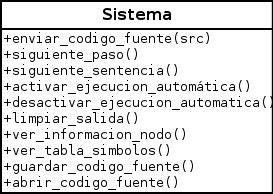
\includegraphics[scale=0.7]{operaciones_sistema_runtree.png} \\
\end{center}
\subsubsection{Operación enviar\_codigo\_fuente}

	\begin{description}
		\item [Nombre:] enviar\_codigo\_fuente (src)
		\item [Responsabilidades:] Envía código fuente para una interpretación por red.
		\item [Referencias Cruzadas: ] Caso de Uso: Enviar código fuente
      \item [Precondiciones:] No tiene.
      \item [Postcondiciones:] \hfill
      \begin {itemize}
         \item Se creó un ``tree'' ``t'' a partir del código enviado a interpretación (creación de objeto).
         \item Se creó un conjunto ``$n_0...n_n$'' de ``node'' a partir de los datos recibidos de la petición (creación de objeto).
         \item Se asoció ``$n_i\ \epsilon\ n_0...n_n$'' a ``$n_k\ \epsilon\ n_0...n_n$'' para construir el árbol sintáctico (creación de enlace).
         \item Se asoció  ``$n_r\ \epsilon\ n_0...n_n$'', raíz del árbol sintáctico, al ``tree'' ``t'' (creación de enlace).
         \item Se inicializó el atributo ``canvas'' del ``tree'' `t'' para dibujar el árbol correspondiente a los nodos ``$\ n_0...n_n$''.
         \item Se creó un ``symbols'' ``s'' (creación de objeto).
         \item Se creó tres instancias de ``table'': ``vars'', ``funcs'' y ``class'' (creación de objeto).
         \item Se asociarón ``vars'', ``funcs'' y ``class'' a ``s'' (creación de enlace).
      \end{itemize}
	\end{description}


\subsubsection{Operación siguiente\_paso}

	\begin{description}
		\item [Nombre:] siguiente\_paso
		\item [Responsabilidades:] Obtiene el siguiente paso del proceso de interpretación abierto.
		\item [Referencias Cruzadas: ] Caso de Uso: Siguiente paso
      \item [Precondiciones:] \hfill
         \begin {itemize}
         \item Se creó un ``tree'' ``t''.
         \item Se creó un conjunto ``$n_0...n_n$'' de ``node''.
         \item Se asoció ``$n_i\ \epsilon\ n_0...n_n$'' a ``$n_k\ \epsilon\ n_0...n_n$'' para construir el árbol sintáctico.
         \item Se asoció  ``$n_r\ \epsilon\ n_0...n_n$'', raíz del árbol sintáctico, al ``tree'' ``t''.
         \item Se creó un ``symbols'' ``s''.
         \item Se creó tres instancias de ``table'': ``vars'', ``funcs'' y ``class''.
         \item Se asociarón ``vars'', ``funcs'' y ``class'' a ``s''.
      \end{itemize}
      \item [Postcondiciones:] \hfill
      \begin {itemize}
         \item Se creó el conjunto ``$r_0...r_n$'' de `refs'' según el nuevo paso del proceso de interpretación (creación de objeto).
         \item Se creó el conjunto ``$v_0...v_m$'' de `node'' correspondiente a los valores generados en el paso del proceso de interpretación (creación de objeto).
         \item Se asoció ``$v_i$'' a ``$r_i$'' como valor de la refercia (creación de enlace).
         \item Se asoció ``$r_i\ \epsilon \ r_0...r_n$'' a ``vars'', ``funcs'' o ``class'' según el paso del proceso de interpretación (creación de enlace).  
         \item Se actualizó el valor del atributo ``canvas'' de ``s'' para reflejar el nuevo estado tras la ejecución del paso.
         \item Se actualizó el valor del atributo ``canvas'' de ``t'' para reflejar el nuevo estado tras la ejecución del paso.
      \end{itemize}
	\end{description}


\subsubsection{Operación siguiente\_sentencia}

	\begin{description}
		\item [Nombre:] siguiente\_sentencia
		\item [Responsabilidades:] Obtiene la siguiente sentencia dentro del proceso de interpretación abierto.
		\item [Referencias Cruzadas: ] Caso de Uso: Siguiente sentencia
      \item [Precondiciones:] \hfill
         \begin {itemize}
         \item Se creó un ``tree'' ``t''.
         \item Se creó un conjunto ``$n_0...n_n$'' de ``node''.
         \item Se asoció ``$n_i\ \epsilon\ n_0...n_n$'' a ``$n_k\ \epsilon\ n_0...n_n$'' para construir el árbol sintáctico.
         \item Se asoció  ``$n_r\ \epsilon\ n_0...n_n$'', raíz del árbol sintáctico, al ``tree'' ``t''.
         \item Se creó un ``symbols'' ``s''.
         \item Se creó tres instancias de ``table'': ``vars'', ``funcs'' y ``class''.
         \item Se asociarón ``vars'', ``funcs'' y ``class'' a ``s''.
      \end{itemize}
      \item [Postcondiciones:] \hfill
      \begin {itemize}
         \item Se creó el conjunto ``$r_0...r_n$'' de `refs'' según la nueva sentencia interpretada (creación de objeto).
         \item Se creó el conjunto ``$v_0...v_m$'' de `node'' correspondiente a los valores generados en la sentencia  interpretada (creación de objeto).
         \item Se asoció ``$v_i$'' a ``$r_i$'' como valor de la refercia (creación de enlace).
         \item Se asoció ``$r_i\ \epsilon \ r_0...r_n$'' a ``vars'', ``funcs'' o ``class'' según la sentencia interpretada (creación de enlace).  
         \item Se actualizó el valor del atributo ``canvas'' de ``s'' para reflejar el nuevo estado tras la ejecución de la sentencia.
         \item Se actualizó el valor del atributo ``canvas'' de ``t'' para reflejar el nuevo estado tras la ejecución del la sentencia.
      \end{itemize}
	\end{description}


\subsubsection{Operación activar\_ejecucion\_automatica}

	\begin{description}
		\item [Nombre:] activar\_ejecucion\_automatica
		\item [Responsabilidades:] Activa la ejecución automática del proceso de interpretación.
		\item [Referencias Cruzadas: ] Caso de Uso: Activar ejecución automática
      \item [Precondiciones:] \hfill
         \begin {itemize}
         \item Se creó un ``tree'' ``t''.
         \item Se creó un conjunto ``$n_0...n_n$'' de ``node''.
         \item Se asoció ``$n_i\ \epsilon\ n_0...n_n$'' a ``$n_k\ \epsilon\ n_0...n_n$'' para construir el árbol sintáctico.
         \item Se asoció  ``$n_r\ \epsilon\ n_0...n_n$'', raíz del árbol sintáctico, al ``tree'' ``t''.
         \item Se creó un ``symbols'' ``s''.
         \item Se creó tres instancias de ``table'': ``vars'', ``funcs'' y ``class''.
         \item Se asociarón ``vars'', ``funcs'' y ``class'' a ``s''.
      \end{itemize}
      \item [Postcondiciones:] \hfill
      \begin {itemize}
         \item Se establece a ``1'' el atributo ``auto'' de ``t''.
      \end{itemize}
	\end{description} 


\subsubsection{Operación desactivar\_ejecucion\_automatica}

	\begin{description}
		\item [Nombre:] desactivar\_ejecucion\_automatica
		\item [Responsabilidades:] Desactiva la ejecución automática del proceso de interpretación.
		\item [Referencias Cruzadas: ] Caso de Uso: Desactivar ejecución automática
      \item [Precondiciones:] \hfill
         \begin {itemize}
         \item Se creó un ``tree'' ``t''.
         \item Se creó un conjunto ``$n_0...n_n$'' de ``node''.
         \item Se asoció ``$n_i\ \epsilon\ n_0...n_n$'' a ``$n_k\ \epsilon\ n_0...n_n$'' para construir el árbol sintáctico.
         \item Se asoció  ``$n_r\ \epsilon\ n_0...n_n$'', raíz del árbol sintáctico, al ``tree'' ``t''.
         \item Se creó un ``symbols'' ``s''.
         \item Se creó tres instancias de ``table'': ``vars'', ``funcs'' y ``class''.
         \item Se asociarón ``vars'', ``funcs'' y ``class'' a ``s''.
      \end{itemize}
      \item [Postcondiciones:] \hfill
      \begin {itemize}
         \item Se establece a ``0'' el atributo ``auto'' de ``t''.
      \end{itemize}
	\end{description} 


\subsubsection{Operación limpiar\_salida}

	\begin{description}
		\item [Nombre:] limpiar\_salida
		\item [Responsabilidades:] Limpia la salida producida por el proceso de interpretación
		\item [Referencias Cruzadas: ] Caso de Uso: Limpiar salida
      \item [Precondiciones:] \hfill
         \begin {itemize}
         \item Se creó un ``tree'' ``t''.
         \item Se creó un conjunto ``$n_0...n_n$'' de ``node''.
         \item Se asoció ``$n_i\ \epsilon\ n_0...n_n$'' a ``$n_k\ \epsilon\ n_0...n_n$'' para construir el árbol sintáctico.
         \item Se asoció  ``$n_r\ \epsilon\ n_0...n_n$'', raíz del árbol sintáctico, al ``tree'' ``t''.
         \item Se creó un ``symbols'' ``s''.
         \item Se creó tres instancias de ``table'': ``vars'', ``funcs'' y ``class''.
         \item Se asociarón ``vars'', ``funcs'' y ``class'' a ``s''.
      \end{itemize}
      \item [Postcondiciones:] \hfill
      \begin {itemize}
         \item Se restablece los valores del atributo ``canvas'' de ``t''.
      \end{itemize}
	\end{description} 


\subsubsection{Operación ver\_informacion\_nodo}

	\begin{description}
		\item [Nombre:] ver\_informacion\_nodo
		\item [Responsabilidades:] Muestra la información de un nodo
		\item [Referencias Cruzadas: ] Caso de Uso: Ver información nodo
      \item [Precondiciones:] \hfill
         \begin {itemize}
         \item Se creó un ``tree'' ``t''.
         \item Se creó un conjunto ``$n_0...n_n$'' de ``node''.
         \item Se asoció ``$n_i\ \epsilon\ n_0...n_n$'' a ``$n_k\ \epsilon\ n_0...n_n$'' para construir el árbol sintáctico.
         \item Se asoció  ``$n_r\ \epsilon\ n_0...n_n$'', raíz del árbol sintáctico, al ``tree'' ``t''.
         \item Se creó un ``symbols'' ``s''.
         \item Se creó tres instancias de ``table'': ``vars'', ``funcs'' y ``class''.
         \item Se asociarón ``vars'', ``funcs'' y ``class'' a ``s''.
      \end{itemize}
      \item [Postcondiciones:] \hfill
      \begin {itemize}
         \item Se establece los valores del atributo ``canvas'' de ``t'' para representar la información del nodo.
      \end{itemize}
	\end{description} 


\subsubsection{Operación ver\_tabla\_simbolos}

	\begin{description}
		\item [Nombre:] ver\_tabla\_simbolos
		\item [Responsabilidades:] Muestra la información contenida en una tabla de símbolos
		\item [Referencias Cruzadas: ] Caso de Uso: Ver información nodo
      \item [Precondiciones:] \hfill
         \begin {itemize}
         \item Se creó un ``tree'' ``t''.
         \item Se creó un conjunto ``$n_0...n_n$'' de ``node''.
         \item Se asoció ``$n_i\ \epsilon\ n_0...n_n$'' a ``$n_k\ \epsilon\ n_0...n_n$'' para construir el árbol sintáctico.
         \item Se asoció  ``$n_r\ \epsilon\ n_0...n_n$'', raíz del árbol sintáctico, al ``tree'' ``t''.
         \item Se creó un ``symbols'' ``s''.
         \item Se creó tres instancias de ``table'': ``vars'', ``funcs'' y ``class''.
         \item Se asociarón ``vars'', ``funcs'' y ``class'' a ``s''.
      \end{itemize}
      \item [Postcondiciones:] \hfill
      \begin {itemize}
         \item Se establece los valores del atributo ``canvas'' de ``s'' para representar la información de la tabla de símbolos.
      \end{itemize}
	\end{description} 



